\documentclass[12pt,a4paper]{article}

\usepackage[T2A]{fontenc}
\usepackage[utf8]{inputenc}
\usepackage[russian]{babel}
\usepackage[a4paper,margin=2.2cm]{geometry}
\usepackage{amsmath,amssymb}
\usepackage{booktabs}
\usepackage{tabularx}
\usepackage{array}
\usepackage{graphicx}
\usepackage{float}
\usepackage{caption}
\usepackage{multirow}
\usepackage{enumitem}
\usepackage{setspace}
\usepackage{titlesec}

\setlength{\parindent}{1.25cm}
\setlength{\parskip}{0.3em}
\onehalfspacing
\pagestyle{plain}
\captionsetup{font=small, labelfont=bf}
\titleformat{\section}{\large\bfseries}{\thesection.}{0.5em}{}
\titleformat{\subsection}{\normalsize\bfseries}{\thesubsection.}{0.5em}{}

\newcommand{\num}[1]{#1}
\newcommand{\hypnull}{\mathrm{H}_0}
\newcommand{\hypalt}{\mathrm{H}_1}

\begin{document}

\begin{titlepage}
\thispagestyle{empty}
\begin{center}
{\bfseries Университет ИТМО \par}
{\bfseries Мегафакультет компьютерных технологий и управления \par}
{\bfseries Факультет программной инженерии и компьютерной техники \par}

\vspace{5cm}

{\Large\bfseries ОТЧЁТ ПО РГР №2\par}
\vspace{0.5cm}
{\Large\bfseries Проверка статистических гипотез\par}

\vfill
\end{center}

\begin{flushright}
\begin{tabular}{ll}
Преподаватель: & Селина Елена Георгиевна \\
Студенты: & Деревянко Владимир Владимирович \\
 & Лоскутов Прохор Александрович \\
 & Стивен Франклин Фейвор \\
\end{tabular}
\end{flushright}
\end{titlepage}

\section{Введение и исходные данные}

В работе используется файл \texttt{resources/RGR2\_A-1\_X1-X4.csv}. Объём выборки равен $n=\num{108}$, уровень значимости принят равным $\alpha=\num{0.05}$, единицы измерения --- мс.

Проверяются следующие гипотезы:
\begin{enumerate}[label=\arabic*.]
\item для выборок $X_1$ и $X_2$ --- гипотеза о равенстве математических ожиданий двух независимых нормальных совокупностей;
\item для выборки $X_3$ --- гипотеза $\hypnull\colon \mu=\num{62.55}$;
\item для выборки $X_4$ --- гипотеза $\hypnull\colon X_4 \sim \mathrm{Exp}(\lambda=\num{0.085})$;
\item дополнительно для $X_1$ и $X_2$ применяется непараметрический критерий Манна--Уитни.
\end{enumerate}

\subsection{Описательная статистика}

\begin{table}[H]
\centering
\small
\caption{Описательная статистика по выборкам}
\setlength{\tabcolsep}{5pt}
\begin{tabular}{lrrrrrrrr}
\toprule
Показатель & $n$ & $\overline{x}$ & $s$ & $\min$ & $Q_{0.25}$ & $\mathrm{Me}$ & $Q_{0.75}$ & $\max$ \\
\midrule
$X_1$ & 108 & 81.822 & 9.734 & 60.370 & 74.690 & 82.410 & 89.118 & 100.300 \\
$X_2$ & 108 & 85.858 & 9.037 & 67.610 & 79.145 & 84.960 & 92.538 & 115.840 \\
$X_3$ & 108 & 61.305 & 8.121 & 36.510 & 57.045 & 61.150 & 65.575 & 86.580 \\
$X_4$ & 108 & 11.247 & 11.022 & 0.010 & 2.930 & 8.460 & 16.645 & 72.170 \\
\bottomrule
\end{tabular}
\end{table}

\begin{figure}[H]
\centering
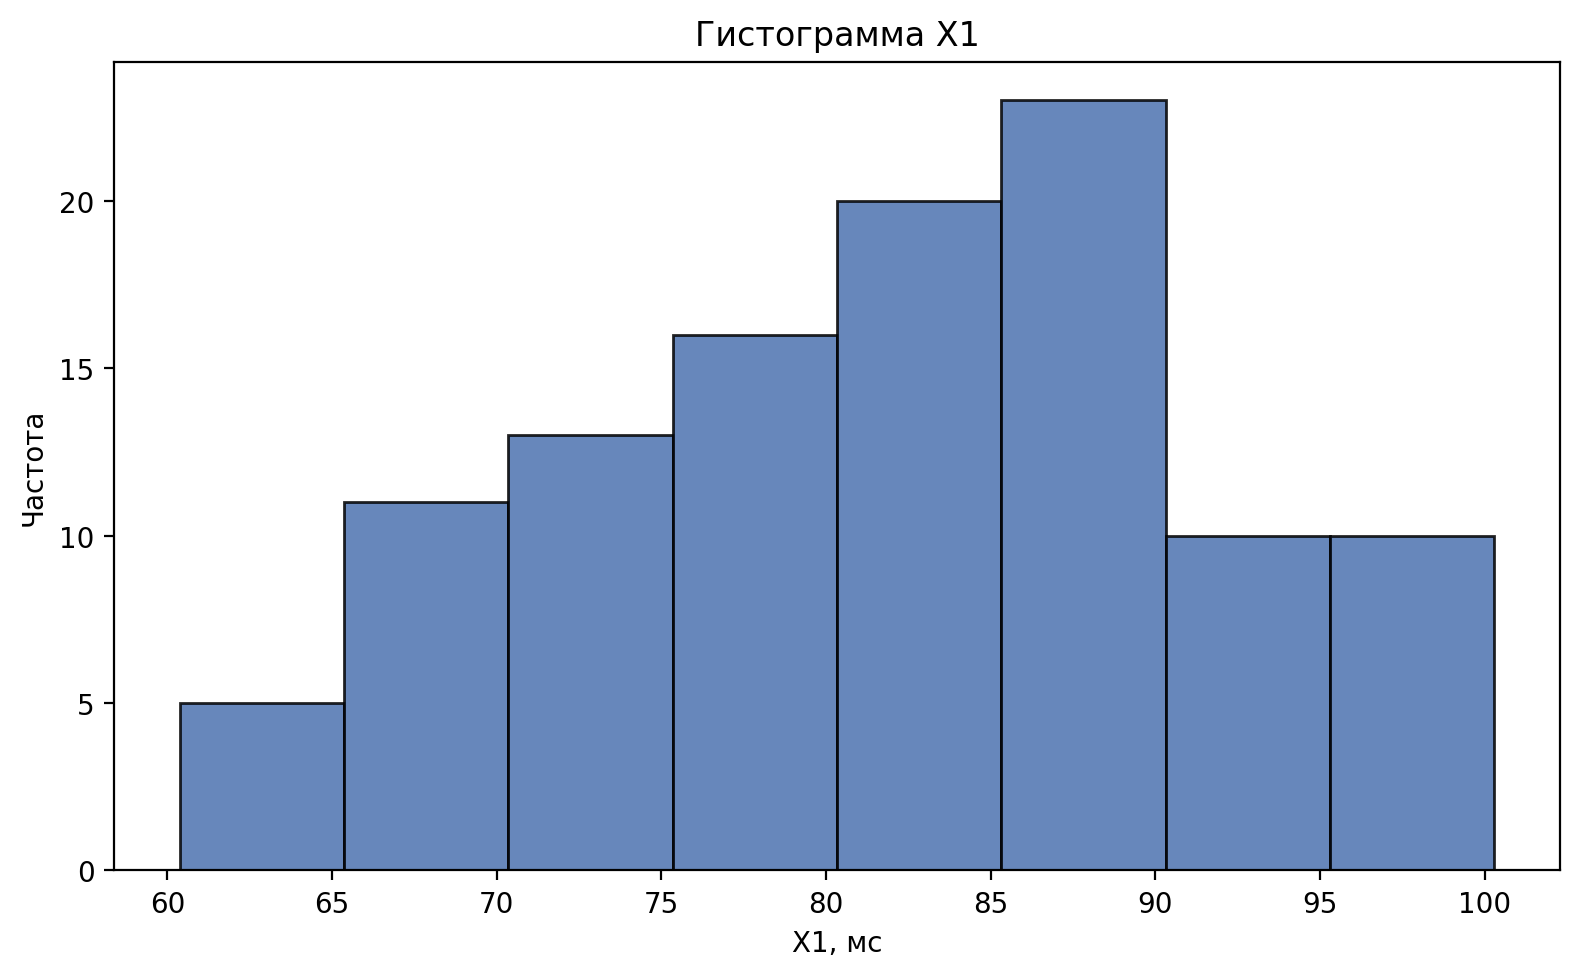
\includegraphics[width=0.72\textwidth]{figures/x1_hist.png}
\caption{Гистограмма выборки $X_1$}
\end{figure}

\begin{figure}[H]
\centering
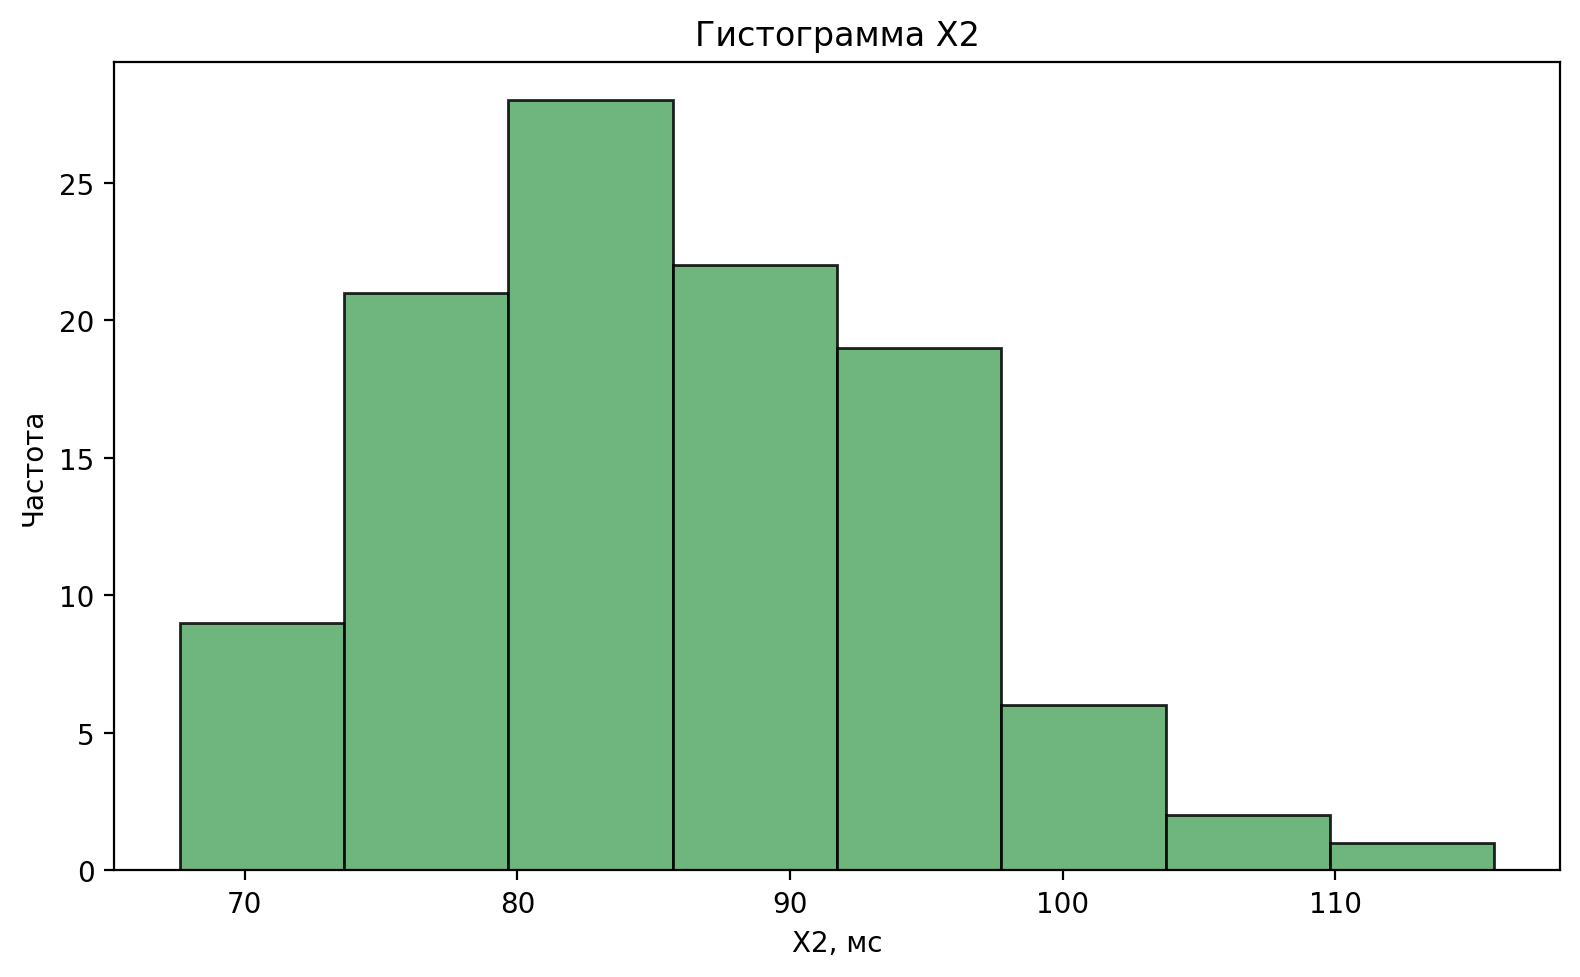
\includegraphics[width=0.72\textwidth]{figures/x2_hist.png}
\caption{Гистограмма выборки $X_2$}
\end{figure}

\begin{figure}[H]
\centering
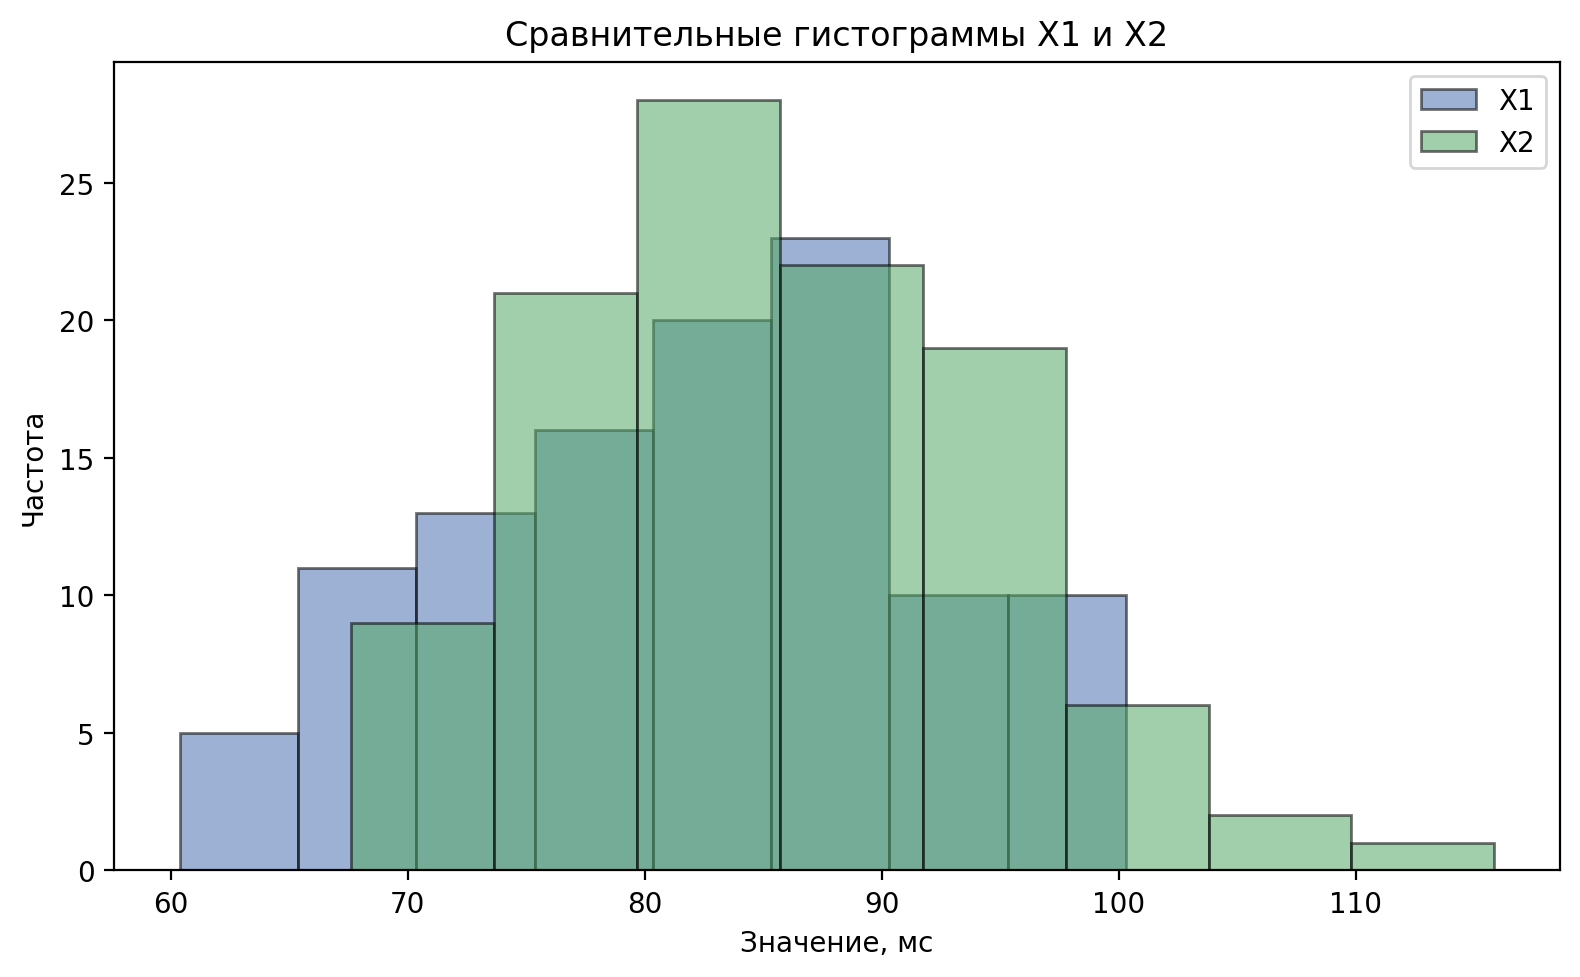
\includegraphics[width=0.82\textwidth]{figures/x1_x2_comparison_hist.png}
\caption{Сравнительные гистограммы выборок $X_1$ и $X_2$}
\end{figure}

\begin{figure}[H]
\centering
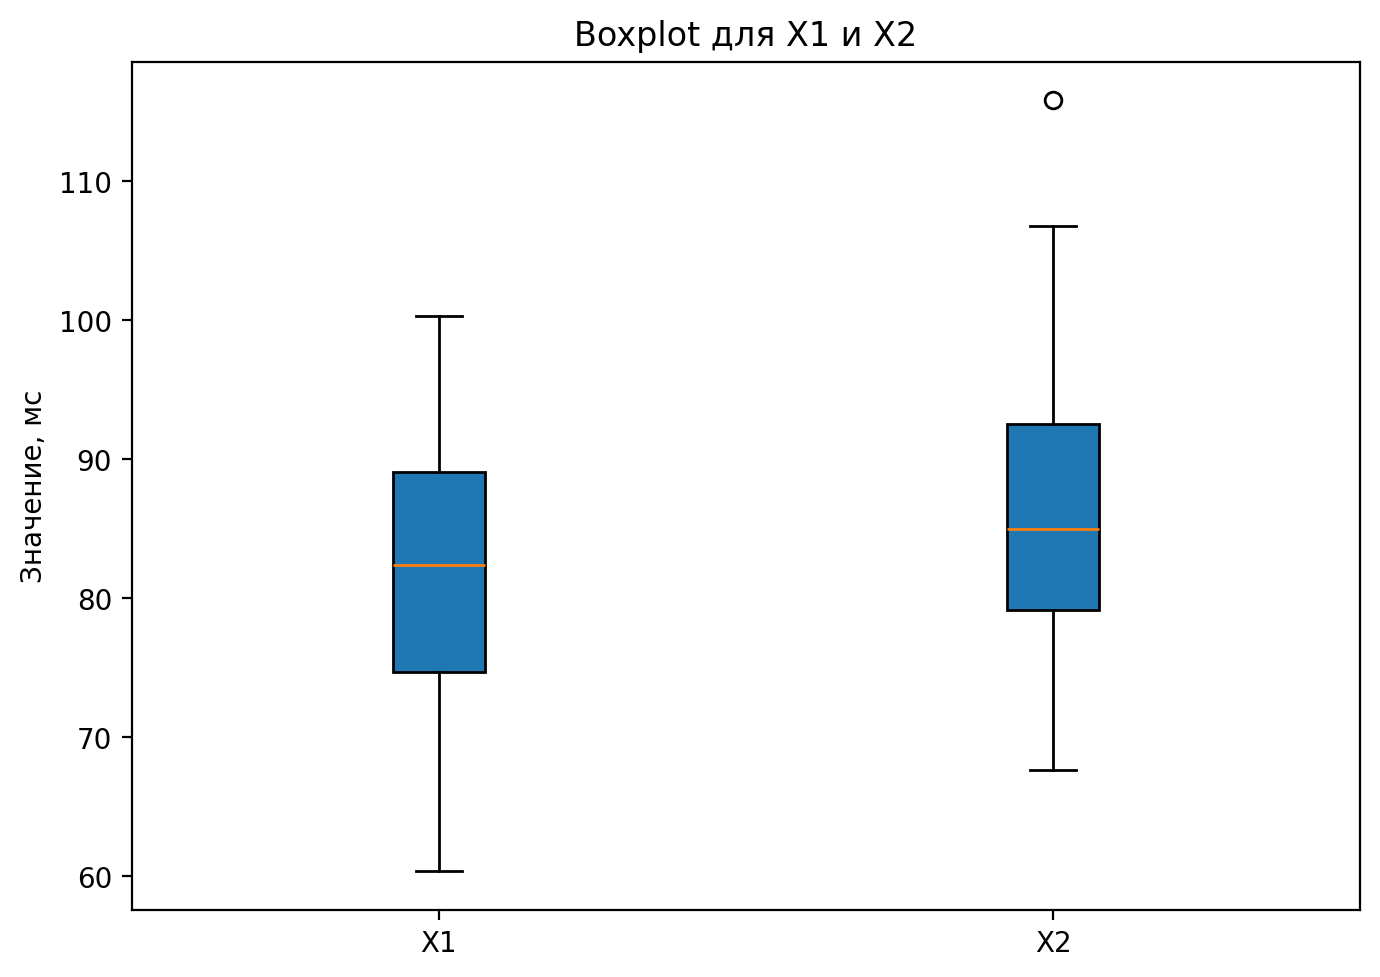
\includegraphics[width=0.62\textwidth]{figures/x1_x2_boxplot.png}
\caption{Диаграмма размаха для $X_1$ и $X_2$}
\end{figure}

\section{Проверка гипотезы о равенстве математических ожиданий $X_1$ и $X_2$}

Формулируются гипотезы
\[
\hypnull\colon \mu_{X_1}=\mu_{X_2}, \qquad
\hypalt\colon \mu_{X_1}\neq \mu_{X_2}.
\]

Используется двухвыборочный t-критерий Стьюдента для независимых выборок. Его применение соответствует условию задачи, где рассматриваются две независимые нормальные совокупности.

Статистика критерия:
\[
t_{\text{набл}}=
\frac{\overline{x}_1-\overline{x}_2}
{s_p \sqrt{\frac{1}{n_1}+\frac{1}{n_2}}},
\qquad
s_p^2=\frac{(n_1-1)s_1^2+(n_2-1)s_2^2}{n_1+n_2-2}.
\]

По данным выборки:
\[
\overline{x}_1=\num{81.822}, \quad
\overline{x}_2=\num{85.858}, \quad
s_1^2=\num{94.758}, \quad
s_2^2=\num{81.658},
\]
\[
s_p^2=\num{88.208}, \quad
t_{\text{набл}}=\num{-3.158}, \quad
\nu=n_1+n_2-2=\num{214}.
\]

Критическое значение для двусторонней альтернативы равно
\[
t_{1-\alpha/2;\nu}=t_{0.975;214}=\num{1.971}.
\]

Также вычислено $p$-value:
\[
p=\num{0.001818}.
\]

Так как $|t_{\text{набл}}|>\num{1.971}$ и $p<\alpha$, нулевая гипотеза отвергается. Следовательно, статистически значимое различие между математическими ожиданиями выборок $X_1$ и $X_2$ обнаружено.

Ошибка первого рода в этом пункте состоит в том, чтобы сделать вывод о различии средних, хотя в действительности математические ожидания совпадают.

\section{Проверка гипотезы по $X_3$}

Проверяются гипотезы
\[
\hypnull\colon \mu=\num{62.55}, \qquad
\hypalt\colon \mu\neq \num{62.55}.
\]

Используется одновыборочный t-критерий Стьюдента для нормального распределения с неизвестной дисперсией. Статистика имеет вид
\[
t_{\text{набл}}=\frac{\overline{x}-\mu_0}{s/\sqrt{n}}.
\]

Для рассматриваемой выборки:
\[
\overline{x}=\num{61.305}, \quad
s=\num{8.121}, \quad
\frac{s}{\sqrt{n}}=\num{0.781}, \quad
t_{\text{набл}}=\num{-1.593}, \quad
\nu=n-1=\num{107}.
\]

Критическое значение равно
\[
t_{1-\alpha/2;\nu}=t_{0.975;107}=\num{1.982},
\]
а $p$-value равно
\[
p=\num{0.114033}.
\]

Поскольку $|t_{\text{набл}}|<\num{1.982}$ и $p>\alpha$, оснований отвергать гипотезу $\hypnull$ нет. Выборка $X_3$ не противоречит предположению о математическом ожидании $\mu=\num{62.55}$.

Ошибка первого рода здесь означает отклонение гипотезы $\hypnull$, хотя фактически математическое ожидание действительно равно \num{62.55}.

\begin{figure}[H]
\centering
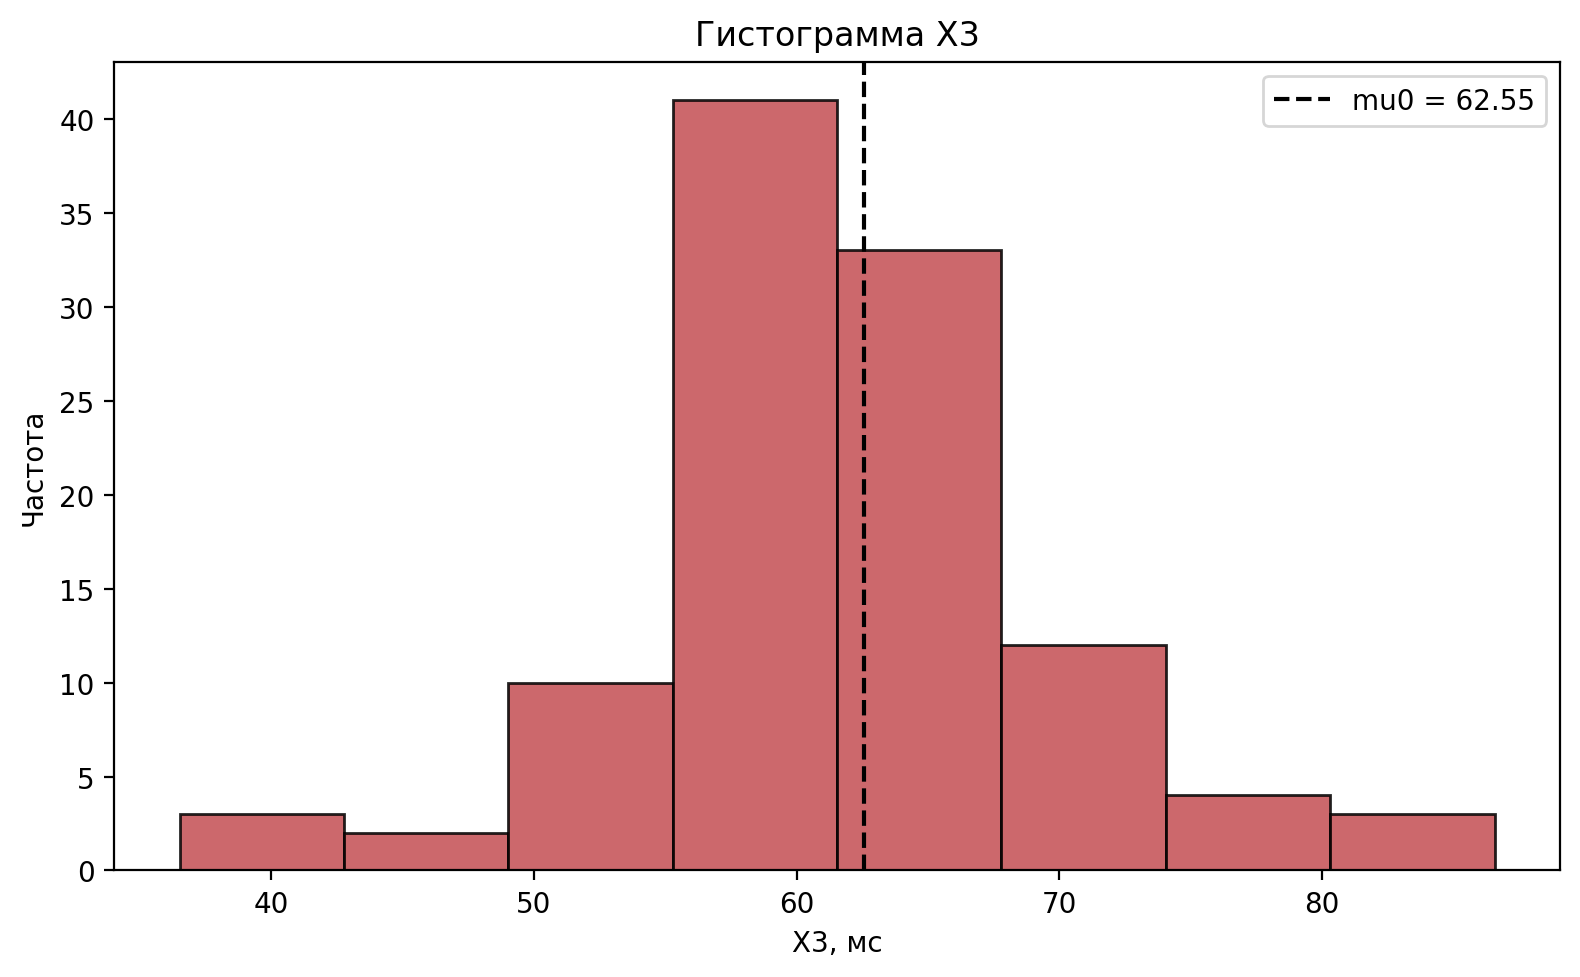
\includegraphics[width=0.72\textwidth]{figures/x3_hist.png}
\caption{Гистограмма выборки $X_3$}
\end{figure}

\section{Непараметрический критерий для $X_1$ и $X_2$}

Для тех же выборок дополнительно применён критерий Манна--Уитни. Проверяются гипотезы
\[
\hypnull\colon F_{X_1}(x)=F_{X_2}(x), \qquad
\hypalt\colon F_{X_1}(x)\neq F_{X_2}(x).
\]

В основе критерия лежит статистика
\[
U = R_1 - \frac{n_1(n_1+1)}{2},
\]
где $R_1$ --- сумма рангов элементов первой выборки.

По данным получено
\[
U_{\text{набл}}=\num{4633}, \qquad p=\num{0.009065}.
\]

Так как $p<\alpha$, нулевая гипотеза отвергается. Вывод совпадает с результатом параметрического t-критерия: выборки $X_1$ и $X_2$ различаются по положению.

Совпадение выводов параметрического и непараметрического критериев объясняется тем, что различие между выборками выражено достаточно отчётливо и обнаруживается обеими процедурами.

Ошибка первого рода в этом пункте --- сделать вывод о различии положений распределений, хотя в действительности различия отсутствуют.

\section{Критерий согласия Пирсона для $X_4$}

Проверяются гипотезы
\[
\hypnull\colon X_4 \sim \mathrm{Exp}(\lambda=\num{0.085}), \qquad
\hypalt\colon X_4 \not\sim \mathrm{Exp}(\lambda=\num{0.085}).
\]

Используется критерий согласия Пирсона. Теоретические вероятности по интервалам вычисляются по формуле
\[
p_i = F(b_i)-F(a_i),
\]
где для показательного распределения
\[
F(x)=1-e^{-\lambda x}, \qquad x\ge 0.
\]

Ожидаемые частоты равны
\[
E_i=np_i,
\]
а статистика критерия имеет вид
\[
\chi^2_{\text{набл}}=\sum_{i=1}^{k}\frac{(O_i-E_i)^2}{E_i}.
\]

После начального разбиения интервалы были объединены так, чтобы во всех группах ожидаемая частота была не меньше \num{5}. Параметр $\lambda$ задан в условии и по выборке не оценивался, поэтому число степеней свободы равно $k-1$.

\begin{table}[H]
\centering
\small
\caption{Интервалы для критерия Пирсона по выборке $X_4$}
\setlength{\tabcolsep}{5pt}
\begin{tabularx}{\textwidth}{>{\raggedright\arraybackslash}p{3.5cm}rrrr}
\toprule
Интервал & $O_i$ & $E_i$ & $p_i$ & $\frac{(O_i-E_i)^2}{E_i}$ \\
\midrule
$[0.000; 10.310)$ & 63 & 63.040 & 0.583700 & 0.000025 \\
$[10.310; 20.620)$ & 24 & 26.243 & 0.242994 & 0.191772 \\
$[20.620; 30.930)$ & 15 & 10.925 & 0.101158 & 1.519869 \\
$[30.930; +\infty)$ & 6 & 7.792 & 0.072147 & 0.412071 \\
\bottomrule
\end{tabularx}
\end{table}

Итоговые значения:
\[
\chi^2_{\text{набл}}=\num{2.124}, \qquad
\nu=k-1=\num{3}, \qquad
\chi^2_{1-\alpha;\nu}=\chi^2_{0.95;3}=\num{7.815}, \qquad
p=\num{0.547125}.
\]

Так как $\chi^2_{\text{набл}}<\num{7.815}$ и $p>\alpha$, нулевая гипотеза не отвергается. Следовательно, выборка $X_4$ согласуется с показательным распределением с параметром $\lambda=\num{0.085}$.

Ошибка первого рода в этом пункте состоит в отклонении гипотезы о показательном распределении, хотя данные в действительности получены из распределения $\mathrm{Exp}(\num{0.085})$.

\begin{figure}[H]
\centering
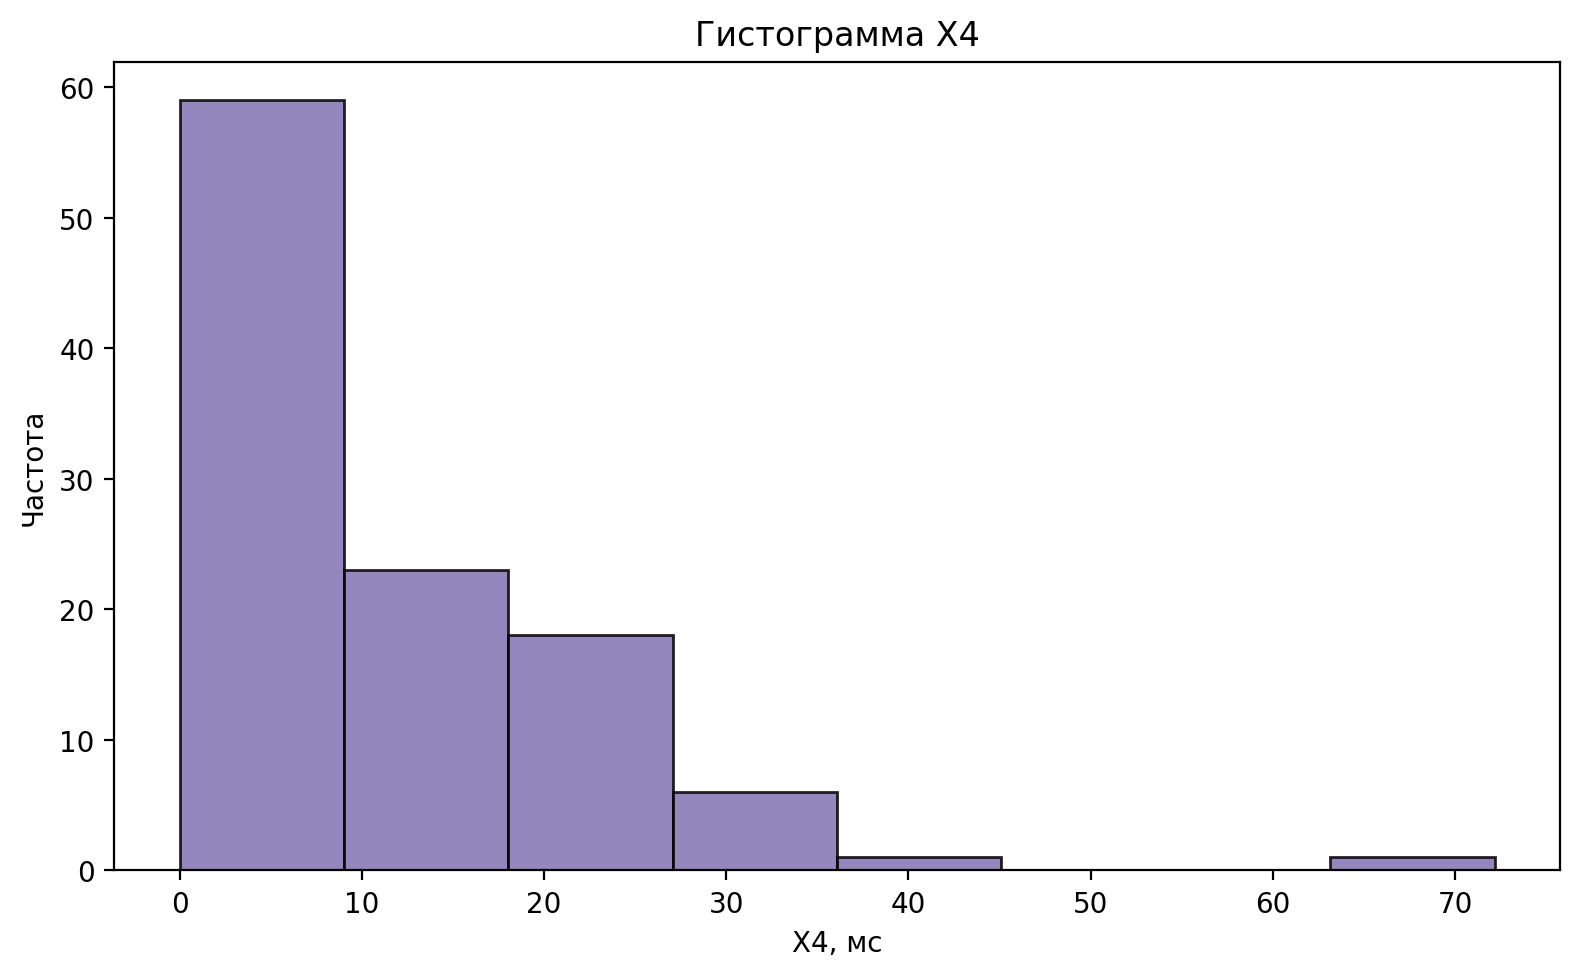
\includegraphics[width=0.72\textwidth]{figures/x4_hist.png}
\caption{Гистограмма выборки $X_4$}
\end{figure}

\begin{figure}[H]
\centering
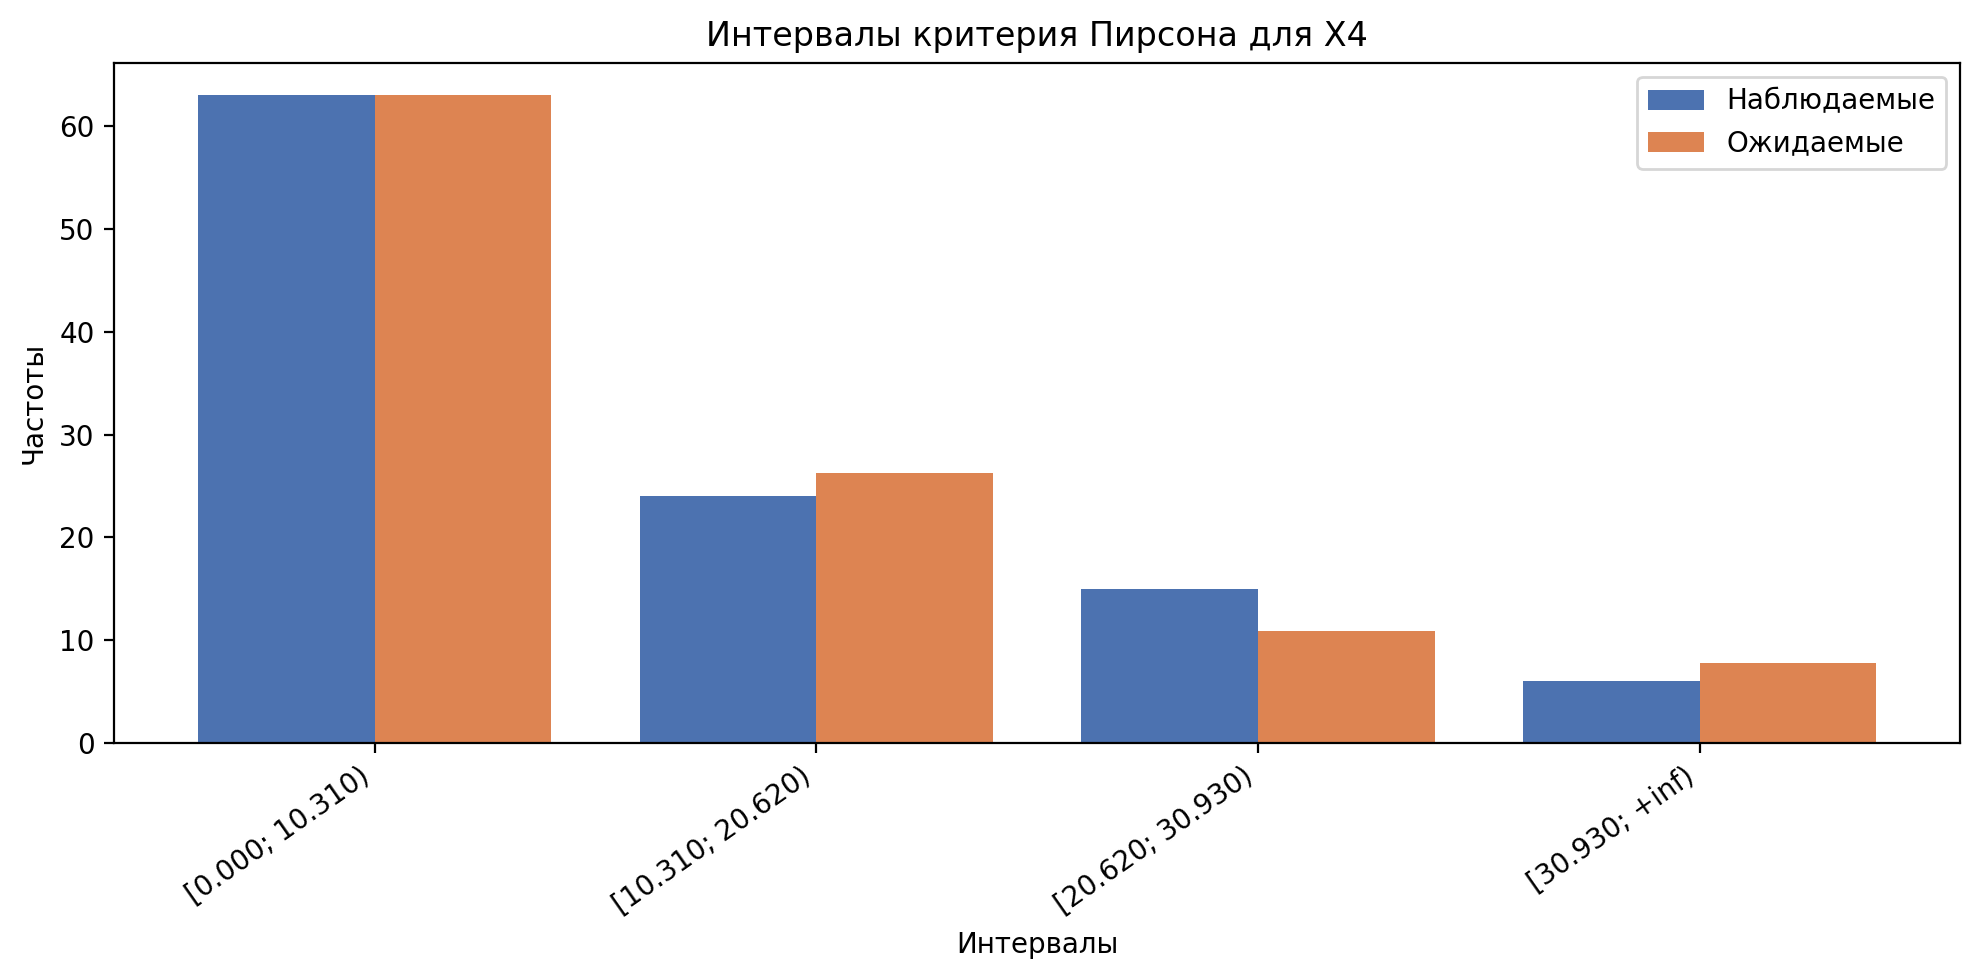
\includegraphics[width=0.9\textwidth]{figures/x4_pearson_intervals.png}
\caption{Наблюдаемые и ожидаемые частоты по интервалам для $X_4$}
\end{figure}

\section{Итоговый вывод}

В работе были проверены гипотезы о равенстве средних для $X_1$ и $X_2$, о значении математического ожидания для $X_3$ и о согласии выборки $X_4$ с показательным распределением. Для этого использовались двухвыборочный и одновыборочный t-критерии Стьюдента, критерий Манна--Уитни и критерий согласия Пирсона.

Для выборок $X_1$ и $X_2$ нулевая гипотеза отвергается как по параметрическому, так и по непараметрическому критерию. Это указывает на статистически значимое различие между выборками. Для $X_3$ оснований отвергать гипотезу $\mu=\num{62.55}$ не получено. Для $X_4$ также не найдено оснований отвергать гипотезу о показательном распределении с параметром $\lambda=\num{0.085}$.

Таким образом, данные подтверждают различие между $X_1$ и $X_2$, но не противоречат гипотезе о среднем значении выборки $X_3$ и не противоречат гипотезе о показательном распределении выборки $X_4$.

\end{document}
